\section{Reusable Blocks and Convolution Detail}
\label{app:implementation}
The slide appendix presents the architecture through callable PyTorch-style
blocks. The following excerpt preserves that decomposition; it explains the
forward structure rather than replacing the authors' implementation.

\subsection{Callable Units and Shape Contracts}

\begin{lstlisting}
def norm_relu(c):
    return nn.Sequential(nn.BatchNorm2d(c), nn.ReLU())

def unit_2d(c_in, r, c_out):
    conv = nn.Conv2d(c_in, c_out, 3, stride=r, padding=1)
    return nn.Sequential(conv, *norm_relu(c_out))

def unit_2d_initial(c_in, c_out):
    return unit_2d(c_in, 1, c_out)

def unit_2d_keep(c_in):
    return unit_2d(c_in, 1, c_in)

def unit_2d_down(c_in):
    return unit_2d(c_in, 2, 2*c_in)

def decoder_block(c_in, c_out):
    return nn.Sequential(unit_2d_initial(c_in, c_out),
                         unit_2d_keep(c_out))

def upsample_concat(decoder_features, skip_features):
    upsampled_features = F.interpolate(
        decoder_features, scale_factor=2, mode="nearest")
    return torch.cat((upsampled_features, skip_features), dim=1)
\end{lstlisting}

For even input dimensions, an Initial or Keep unit preserves spatial
resolution, while a Down unit halves height and width. More generally, the
kernel-3, padding-1, stride-$r$ convolution gives
$H_{\mathrm{out}}=\lfloor(H_{\mathrm{in}}-1)/r\rfloor+1$, with the analogous
formula for width. The attention pointwise unit instead uses a $1\times1$
convolution to change channels without mixing neighboring spatial cells.
Normalization and activation preserve the tensor shape.

An encoder stage composes two 2D units and, where specified, a pointwise 3D
unit. In this single-frame reconstruction, the 3D helper temporarily inserts
a singleton depth axis, applies a $1\times1\times1$ Conv3d, and flattens that
axis again. It preserves the displayed $H/W/C$ dimensions. Its name is not
evidence of multi-frame temporal aggregation in this forward path.

\noindent\begin{minipage}{\linewidth}
\subsection{The Alignment Code Example}
The project illustrates spatial alignment with a square feature map and a
rotation followed by translation. The excerpt below is the existing
teaching implementation used beside Figure~\ref{fig:rotation-translation}.
It constructs a forward transform, inverts it for output-to-input sampling,
and applies the same grid to every channel.

\lstinputlisting[firstline=4]{assets/final/graph/feature_alignment_example_v1.py}
\end{minipage}

The example's $x$ coordinate points right and $y$ points down. Translation
is expressed in cells of this small feature grid. The factors $2/W$ and
$2/H$ convert displacements to the normalized grid coordinates used by
the sampler. The example call is
\begin{lstlisting}
aligned_features = align_features(
    sender_features, angle_deg=90, dx=1, dy=1)
\end{lstlisting}
The original model's pose handling and scale conversion remain part of
its implementation; this small example isolates the sampling operation.

\FloatBarrier
\subsection{Numerical Input and Kernel Dimensions}
The separate convolution walkthrough uses a video tensor with three frames,
three channels, height three, and width four. Figure~\ref{fig:conv-input}
shows all values. Channel colors remain fixed across frames, making it
possible to track a spatial patch through the numerical calculation.

\begin{figure}[htbp]
\centering
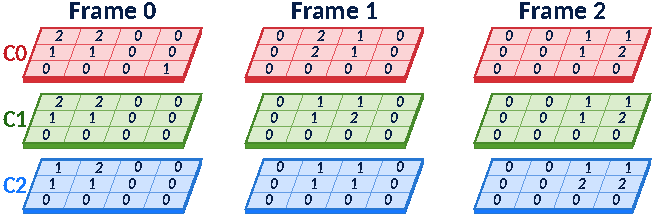
\includegraphics[width=\linewidth]{convolution/conv-palette-v2-inputs.pdf}
\caption[The three-frame, three-channel convolution input]{The project's
numerical tensor example. Columns are frames; colors distinguish channels
C0, C1, and C2. Each channel plane has three rows and four columns.}
\label{fig:conv-input}
\end{figure}

\begin{figure}[htbp]
\centering
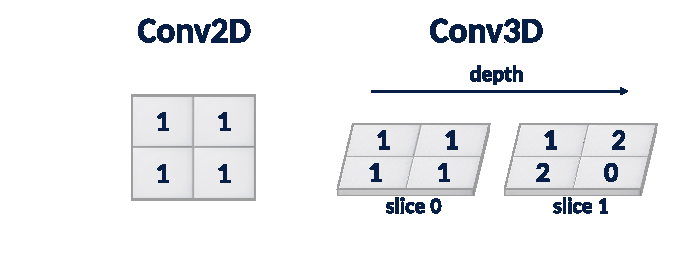
\includegraphics[width=\linewidth]{convolution/conv-palette-v2-kernels-rich-v1.pdf}
\caption[Spatial and temporal kernel slices]{Project kernel illustrations.
The Conv2D spatial kernel contains ones. The Conv3D kernel has two temporal
slices, with different weights in the second slice. Each illustrated
spatial/temporal kernel is applied across the input channels.}
\label{fig:conv-kernels}
\end{figure}

The examples use stride one, no padding, zero bias, and one output channel.
A $2\times2$ spatial kernel on a $3\times4$ plane produces a $2\times3$
output. A Conv3D kernel of depth two on three input frames also produces
two output depth slices. Its complete output shape is therefore
$2\times2\times3$ in depth--height--width order.

\FloatBarrier
\subsection{Conv2D: Accumulating Across Channels}
For one output channel, the weight tensor contains a spatial kernel for
every input channel. In this example all those Conv2D weights are one.
At the upper-left output, the four-cell patches of Frame 0 sum to 6 in
C0, 6 in C1, and 5 in C2. The contributions are added:
\[
 y_{0,0}=
 \underbrace{(2+2+1+1)}_{\mathrm{C0}}+
 \underbrace{(2+2+1+1)}_{\mathrm{C1}}+
 \underbrace{(1+2+1+1)}_{\mathrm{C2}}=17.
\]

\begin{figure}[htbp]
\centering
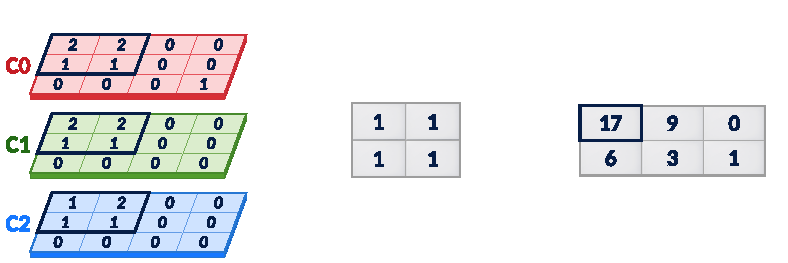
\includegraphics[width=\linewidth]{convolution/conv-palette-v2-conv2d-r0c0-rich-v1.pdf}
\caption[The first Conv2D output and the complete spatial result]{Project
Conv2D example. Outlines select the upper-left patch in each channel;
the highlighted output sums all channel contributions.}
\label{fig:conv2d-example}
\end{figure}

Sliding the same kernel across Frame 0 gives
\[
 \begin{bmatrix}17&9&0\\6&3&1\end{bmatrix}.
\]
The output is one channel because all three input-channel contributions
feed the same filter. Multiple output channels would use additional learned
filters. Convolving each frame separately does not mix the values of
Frame 0 with those of Frame 1.

\FloatBarrier
\subsection{Conv3D: Accumulating Across Time and Channels}
The temporal kernel in Figure~\ref{fig:conv-kernels} uses
\[
 K_0=\begin{bmatrix}1&1\\1&1\end{bmatrix},\qquad
 K_1=\begin{bmatrix}1&2\\2&0\end{bmatrix}.
\]
The same two-slice pattern is used for each input channel in this teaching
example. At output $(d,r,c)=(0,0,0)$, $K_0$ multiplies the upper-left patch
of Frame 0 and $K_1$ multiplies the corresponding patch of Frame 1. The
recorded arithmetic is
\[
 (6+4)_{\mathrm{C0}}+(6+2)_{\mathrm{C1}}+(5+2)_{\mathrm{C2}}=25.
\]
This calculation combines both temporal slices and all three channels.

\begin{figure}[htbp]
\centering
\newcommand{\ReportConvThreeRow}[3]{%
  \begin{minipage}[c]{0.57\linewidth}
    \centering\small\textbf{#1}\par\smallskip
    \includegraphics[width=\linewidth]{convolution/conv-palette-v2-conv3d-d#2r0c0.pdf}
  \end{minipage}\hfill
  \begin{minipage}[c]{0.19\linewidth}
    \centering\small\textbf{Kernel}\par\smallskip
    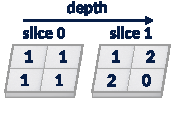
\includegraphics[width=\linewidth]{convolution/conv-palette-v2-kernel3d-rich-v1.pdf}
  \end{minipage}\hfill
  \begin{minipage}[c]{0.20\linewidth}
    \centering\small\textbf{Output: #3}\par\smallskip
    \includegraphics[width=\linewidth]{convolution/conv3d-output-parallelepipeds-v3-d#2r0c0-rich-v1.pdf}
  \end{minipage}%
}
\ReportConvThreeRow{Frames 0 and 1}{0}{$d=0$}\par\bigskip
\ReportConvThreeRow{Frames 1 and 2}{1}{$d=1$}

\caption[Two temporal positions of the Conv3D window]{The project's input
patches, temporal kernel, and output diagrams combined at their original
aspect ratios. Above, Frames 0 and 1 produce 25 at $(0,0,0)$. Below, moving
the temporal window to Frames 1 and 2 produces 8 at $(1,0,0)$.}
\label{fig:conv3d-example}
\end{figure}

Advancing the depth coordinate moves the window to Frames 1 and 2. At
$(1,0,0)$, the three channel contributions become $4+0$, $2+0$, and
$2+0$, giving eight. The complete two output slices in the saved
walkthrough are
\[
 Y_0=\begin{bmatrix}25&27&11\\14&15&5\end{bmatrix},\qquad
 Y_1=\begin{bmatrix}8&21&24\\4&16&20\end{bmatrix}.
\]
Depth and channels are separate axes: the kernel slides over time while
accumulating over channels. This genuine multi-frame example explains
the additional dimension of Conv3D. It should be distinguished from the
architecture's pointwise helper on a singleton depth axis. The complete
sequence of spatial and temporal windows remains in Appendix C of the
presentation.
